\chapter{Fazit}
\label{ch:conclusion}
Im Rahmen der Ihnen vorliegenden Bachelorthesis wurde ein mobile Anwendung entwickelt, die es einem ermöglicht Indoor Maps zu gestalten.
In \autoref{ch:theorybasics} wurde auf die Theorie und die Grundlagen dieser Thesis eingegangen.
Darunter Kartendaten im Allgemeinen, wie man auf diesen zeichnet und welche Typen mobiler Anwendungen es gibt.\pbreak%
%
In \autoref{ch:analysis} wurden im Anschluss die aktuellen Lösungen analysiert.
Dabei wurden Anforderungen aufgestellt, die ein System zur Erstellung von Indoor Maps erfüllen sollte und diese mit den aktuellen Lösungen verglichen.
Dabei wurde etwas genauer auf Geoinformationssysteme eingegangen und die Probleme bei diesen herausgelesen.\pbreak%
%
Nach dem Abschluss der Analyse wurde in \autoref{ch:conception} mit dem Konzept für die Anwendung begonnen.
Zu Beginn des Konzepts wurde ein grobes Design-Konzept erstellt, sodass die unterschiedlichen Komponenten der Anwendung ein ansehnliches und benutzerfreundliches Auftreten haben.
Anschließend wurde dargelegt, wie ein Projekt der Anwendung aufgebaut und gespeichert wird.
Des Weiteren wurde Pläne beschrieben, wie das Bearbeiten der Kartendaten und der Export der erstellten Indoor Maps funktionieren soll.\pbreak%
%
Das \autoref{ch:implementation} hat darauffolgend den Prozess der Implementierung beschrieben und es wurde in \autoref{sec:devios} anfangs auf die Entwicklung auf iOS-Geräten eingegangen.
In diesem Abschnitt wurden die zur Verfügung stehenden Programmiersprachen vorgestellt und ein grober Einblick in die Struktur und den Aufbau eines iOS-Projektes gegeben.
Im \autoref{sec:techimp} wurde dann genauer auf die technische Umsetzung eingegangen.
Dabei wurden besonders die Themen Kodierung der Datenstrukturen und Generics besprochen, sowie genauer auf die Gesture Recognizer eingegangen und welche Probleme bestanden.
Außerdem wude auch beschreiben, warum sich für die programmatische Entwicklung der Benutzeroberfläche entschieden wurde und wie die Elemente auf der angezeigten Karte gezeichnet wurden.\pbreak%
%
Zum Ende des \autoref{ch:implementation} wurde im \autoref{sec:localizing} der Prozess der \Gls{l10n} beschrieben.
Dabei wurde zum Einen auf die bereits existierenden Schnittstellen zum Lokalisieren eingegangen, als auch auf die Problematik bei der Auswahl von Untereinheiten von Regionen bei der Adressauswahl.

\section{\textcolor{red}{Herausforderungen}}
Bei der Entwicklung der Anwendung gab es einige Herausforderungen, die man überwinden musste.
Vor allem das Kodieren der Daten zwischen den \ac{json}-Repräsentationen aus den Dateien und den Datenmodellen in der Anwendung war herausfordernd.

%- Generics
%- MapOverlays
%- Gesture Recognizers
%- ISO Country Codes (IMDF erfordert ein subdivision Identifier)
%- Kein Export und Fehlende Features (zeitlich nicht alle aufgestellten Anforderungen erfüllt)

\section{Analyse der Anwendung}
Im \autoref{ch:analysis} wurden Anforderungen aufgestellt und die aktuelle Situation auf dem Markt analysiert.
Nach Abschluss der Entwicklung findet nun auch ein Abgleich mit den Anforderung bei Indoor Architect statt, sodass das Ergebnis besser bewertet werden kann.

\subsection{Abgleich mit den Anforderungen}
Nach Abschluss der Entwicklung der ersten Version von Indoor Architect kann mit dem Abgleich der Anforderungen begonnen werden.
Für den Vermieter im Anwendungsfall waren die Punkte \emph{Presisliche Stemmbarkeit}, \emph{Schnelle Einarbeitungszeit}, \emph{Leichte und Nachvollziehbare Bedienung} und die \emph{Mobile Nutzung} von Relevanz.
\analysisresults{
Da Indoor Architect nicht monetarisiert wird und der Programmquellcode offen zur Verfügung steht, fallen für die Anwendung selbst keine Kosten an.
Ähnlich wie bei den anylsierten Anwendungen müssen die Geräte für die Nutzung der Software vorhanden sein.
}{
Die Anwendung nutzt an vielen Stellen Beschreibungstexte, die erklären welche Informationen in welchem Format in das entsprechende Feld eingetragen werden müssen.
In den Abbildungen \hyperref[fig:04-address]{A.4}, \hyperref[fig:11-label]{A.11} und \hyperref[fig:13-venue]{A.13} im Anhang kann gesehen werden, wie die Beschreibungstexte dem Anwender näher bringen was eingetragen werden muss.
Das Kennenlernen der Anwendung findet daher nicht über eine externe Dokumentation statt, sondern über das Benutzen der Anwendung selbst.
}{
Beim Benutzen von Indoor Architect wird dem Anwender sofort Rückmeldung über die ausgeführte Aktion gegeben, sodass eine Aktion immer nachvollziehbar ist.
Beim Erstellen von Adressen wird im Hintergrund die Liste der Adressen sofort aktualisiert und bei der Bearbeitung der Kartendaten kann man zu jeder Zeit erkennen, worauf die Anwendung wartet.
}{
Die Anwendung Indoor Architect ist eine iPad-App und kann daher mobil genutzt werden.
Für die Verwaltung der Projekte und die Bearbeitung der Kartendaten wird außerdem keine Internetanbindung benötigt, sodass die Anwendung an jedem Ort genutzt werden kann.
}{
Die entwickelte Anwendung erfüllt die aufgestellten Anforderung in der ersten Entwicklungsversion.
Dabei sollte man bedenken, dass die Erfüllung der Anforderungen ein kontinuierlich fortschreitender Prozess ist.
Bei der Entwicklung neuer Funktionen muss weiter darauf geachtet werden, dass die Einarbeitungszeit kurz gehalten wird und die Bedienung der Funktionen leicht und nachvollziehbar ist.\pbreak%
%
Der aktuelle Stand der entwickelten Anwendung kann noch nicht dafür verwendet werden alle Möglichkeiten des \acl{imdf}s abbilden zu können.
Eine Implementierung aller benötigten Funktionen beansprucht mehr Arbeitszeit, da bei jeder Entwicklung die Anforderungen und die Vorgaben aus dem Design-Konzept eingehalten werden müssen.
}

\subsection{Usability Tests}
Um die Anforderung der schnellen Einarbeitungszeit und der leichten und nachvollziehbaren Bedienung besser einordnen zu können wurde ein Usability Test mit der entwickelten Anwendung durchgeführt.
Die Testpersonen haben eine Liste mit Aufgaben erhalten, die sie innerhalb der Anwendung erfüllen sollten.
Im Anschluss war es ihnen möglich die Benutzung der Anwendung zu bewerten.
Die genauen Aufgabenstellungen und anschließende Bewertungsmöglichkeiten können im \hyperref[sec:appendixc]{Anhang C} eingesehen werden.\pbreak%
%
Bei der Auswertung konnte ermittelt werden, dass von den 11 Testpersonen drei Schwierigkeiten bei der Benutzung der Anwendung vermeldet haben.
Die genau Verteilung der gemeldeten Probleme bei den Aufgaben ist in der Abbildung \ref{fig:usability-column} dargestellt.
\begin{figure}[h]
	\centering
	\vspace{15pt}
	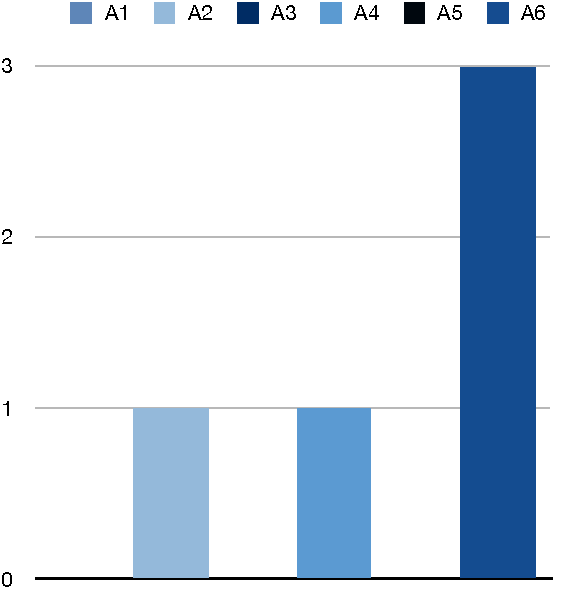
\includegraphics[scale=0.8]{images/usability-results-column.pdf}
	\caption{Benannte Probleme bei den gestellten Aufgaben}
	\label{fig:usability-column}
\end{figure}
Alle drei Personen haben auf eine Schwierigkeit bei der Aufgabe 6 hingewiesen, während zusätzlich bei zweien noch jeweils die Aufgaben 2 und 4 Schwierigkeiten bereitet haben.
Bei der Aufgabe 6 sollten die Benutzer eine Entfernung zwischen zwei Orten messen.
Bei der Bewertung wurde beschrieben, dass nicht klar war wie eine Messung ausgeführt werden kann.
Das lag laut Angaben in erster Linie daran, dass das verwendete Icon die Funktion dahinter nicht klar kommuniziert.
Für eine Optimierung der Usability sollten daher die Icon überprüft und gegebenenfalls ausgewechselt werden.
\section{Ausblick}
In Zukunft kann die Anwendung mit vielen weiteren Funktionen erweitert werden.
Außerdem könnte eine einfache Nutzung einer Anwendung zur Erstellung von Indoor Maps dazu beitragen Indoor Maps weiter zu verbreiten.
Auf diese zwei Punkte wird in diesem Kapitel etwas genau eingegangen.

\subsection{Erweiterbarkeit}
Die Anwendung kann um viele weitere Funktionen erweitert werden.
Einige Funktionen, die nicht essenziell zum Bearbeiten der Kartendaten sind, jedoch den Aufwand deutlich verringern, sind zum Beispiel das automatische erkennen von Eckpunkten, wenn ein Punkt in der nähe gesetzt wurde.
Dadurch könnte man den Vorgang des Hinzufügen von Elementen, die an eine andere anknüpfen deutlich schneller machen.\pbreak
%
Eine weitere geplante Funktion ist die Möglichkeit ein transparentes Bild über die Karte zu legen, wenn man dabei ist die Kartendaten zu bearbeiten.
Dadurch könnte man mit bereits existierenden Bauplänen das Gebäude einfach anhand der transparenten Grafik nachzeichnen und im Anschluss die Detailarbeit vollziehen.\pbreak%
%
Im aktuellen Stand gibt es die Möglichkeit bei jedem Feature einen Kommentar zu hinterlegen.
In einer zukünfitgen Version könnte diese Funktion dahingehen erweitert werden, dass Features auch Tags haben und einer Farbkategorie zugewiesen werden können.
Diese Informationen könnten in die Suche eingebaut werden, sodass nach Tags gesucht werden kann oder nach einer bestimmten Farbkategorie gefiltert werden kann.\pbreak%
%
Besonders in Anwendungen, in denen Inhalte bearbeitet werden, ist es sinnvoll eine Möglichkeit zu bieten die getätigten Änderungen rückgängig zu machen oder zu wiederholen.
Falls bei dem Erstellen eines Polygons ein Fehler unterlaufen ist und man den gezeichneten Punkt rückgängig machen möchte, müsste solch eine Funktion existieren.
Dies ist eine der höher priorisierten Erweiterungen.\pbreak%
%
Das \ac{imdf}-Format definiert in der Spezifikation sehr genau, was valide Daten sind und der in \autoref{ch:conception} im Abschnitt \autoref{sec:validation} erwähnte Audit wäre für die Anwender von Vorteil.
Zwar bietet Apple selbst eine \ac{imdf}-Sandbox an, in welcher man ein \ac{imdf}-Archiv hochladen kann und einfache Fehler angezeigt bekommt und beheben kann, doch eine eingebaute \ac{imdf}-Validierung könnte auch hier Arbeit abnehmen.
Es wäre nicht mehr notwendig das Projekt zu exportieren und im Anschluss in der Sandbox hochzuladen, sondern man könnte eine Validierung direkt in der Anwendung anstoßen und Fehlermeldungen und Lösungsvorschläge erhalten.
Bei einfachen Formfehlern wäre es auch möglich die Probleme automatisch von der Anwendung lösen zu lassen.\pbreak%
%
Neben einem Export wäre es auch sinnvoll einen Import für \ac{imdf}-Archive anzubieten.
Ein bestehendes \ac{imdf}-Archiv könnte von der Anwendung interpretiert werden und zu einem Indoor Architect Projekt umgewandelt werden, sodass jedes \ac{imdf}-Archiv in Indoor Architect bearbeitet werden kann und nicht nur die dort erstellten.

\subsection{\textcolor{red}{Nutzen für Indoor Maps}}
Eine deutlich interessantere Frage ist jedoch, ob eine einfach zu bedienende Anwendung einen Nutzen für Indoor Maps im Allgemeinen oder deren Verbreitung hat.
